\chapter{Guidance Assessment}\label{Ch:NumericalAssessment}

\section{Reference Trajectory Optimization}
In this section we solve the ROGP for a variety of objective weights $(w_h,\,w_s)$ while holding the gains constant. This demonstrates the extent to which the reference trajectory can impact the solution for a fixed set of gains. In the first subsection, we consider the open-loop ($K=\zero$) scenario to gauge the level of dispersions that must be mitigated by the entry guidance, and the extent to which open-loop covariance shaping can help. MSL entry guidance designers performed a similar exercise~\cite{MSL_EDL2}. The second subsection repeats the sweep over the weights in a closed-loop scenario.

\subsection{Open-Loop Optimization}
Figure~\ref{Fig:MCResultsOpenLoop} presents contours of the Monte Carlo estimated 3$\sigma$-low altitude and range errors. The 3$\sigma$ range errors vary from 59 to 66 km, while the 3$\sigma$-low altitude varies from 7.8 km to 10.6 km. Increasing the weight $w_s$ reduces range errors as intended but comes at a penalty to altitude performance. The results also highlight the magnitude of the terminal state variations arising from the variations in the initial state and model uncertainty. 
%TODO: Show some control profiles? 
\begin{figure}[h!]
	\centering
	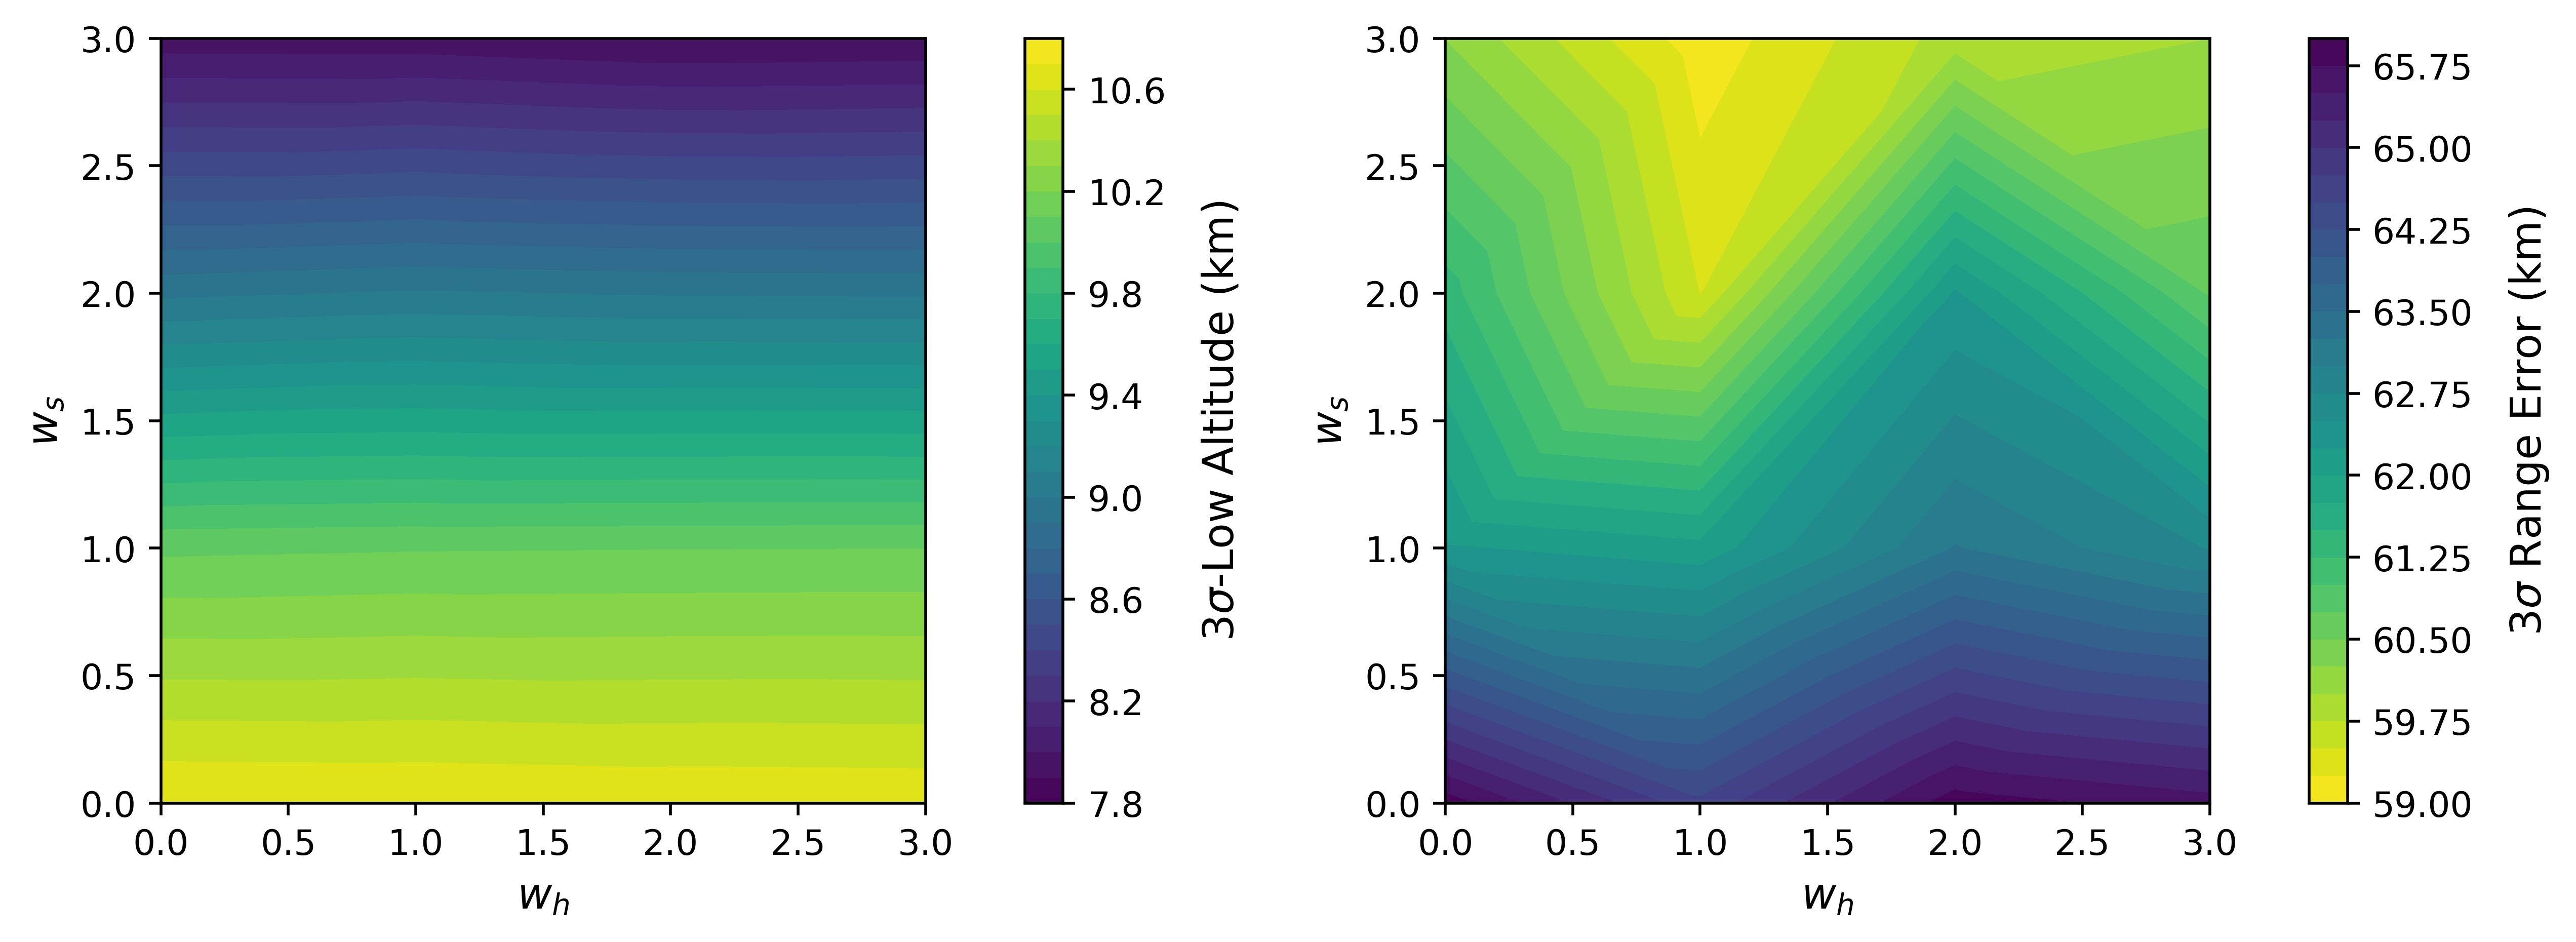
\includegraphics[width=1\textwidth]{Images/OpenLoop_WeightSweepMCResults}
	\caption{Monte Carlo statistics for the open-loop trajectory optimization. }
	\label{Fig:MCResultsOpenLoop}
\end{figure}
%\begin{figure}[h!]
%	\centering
%	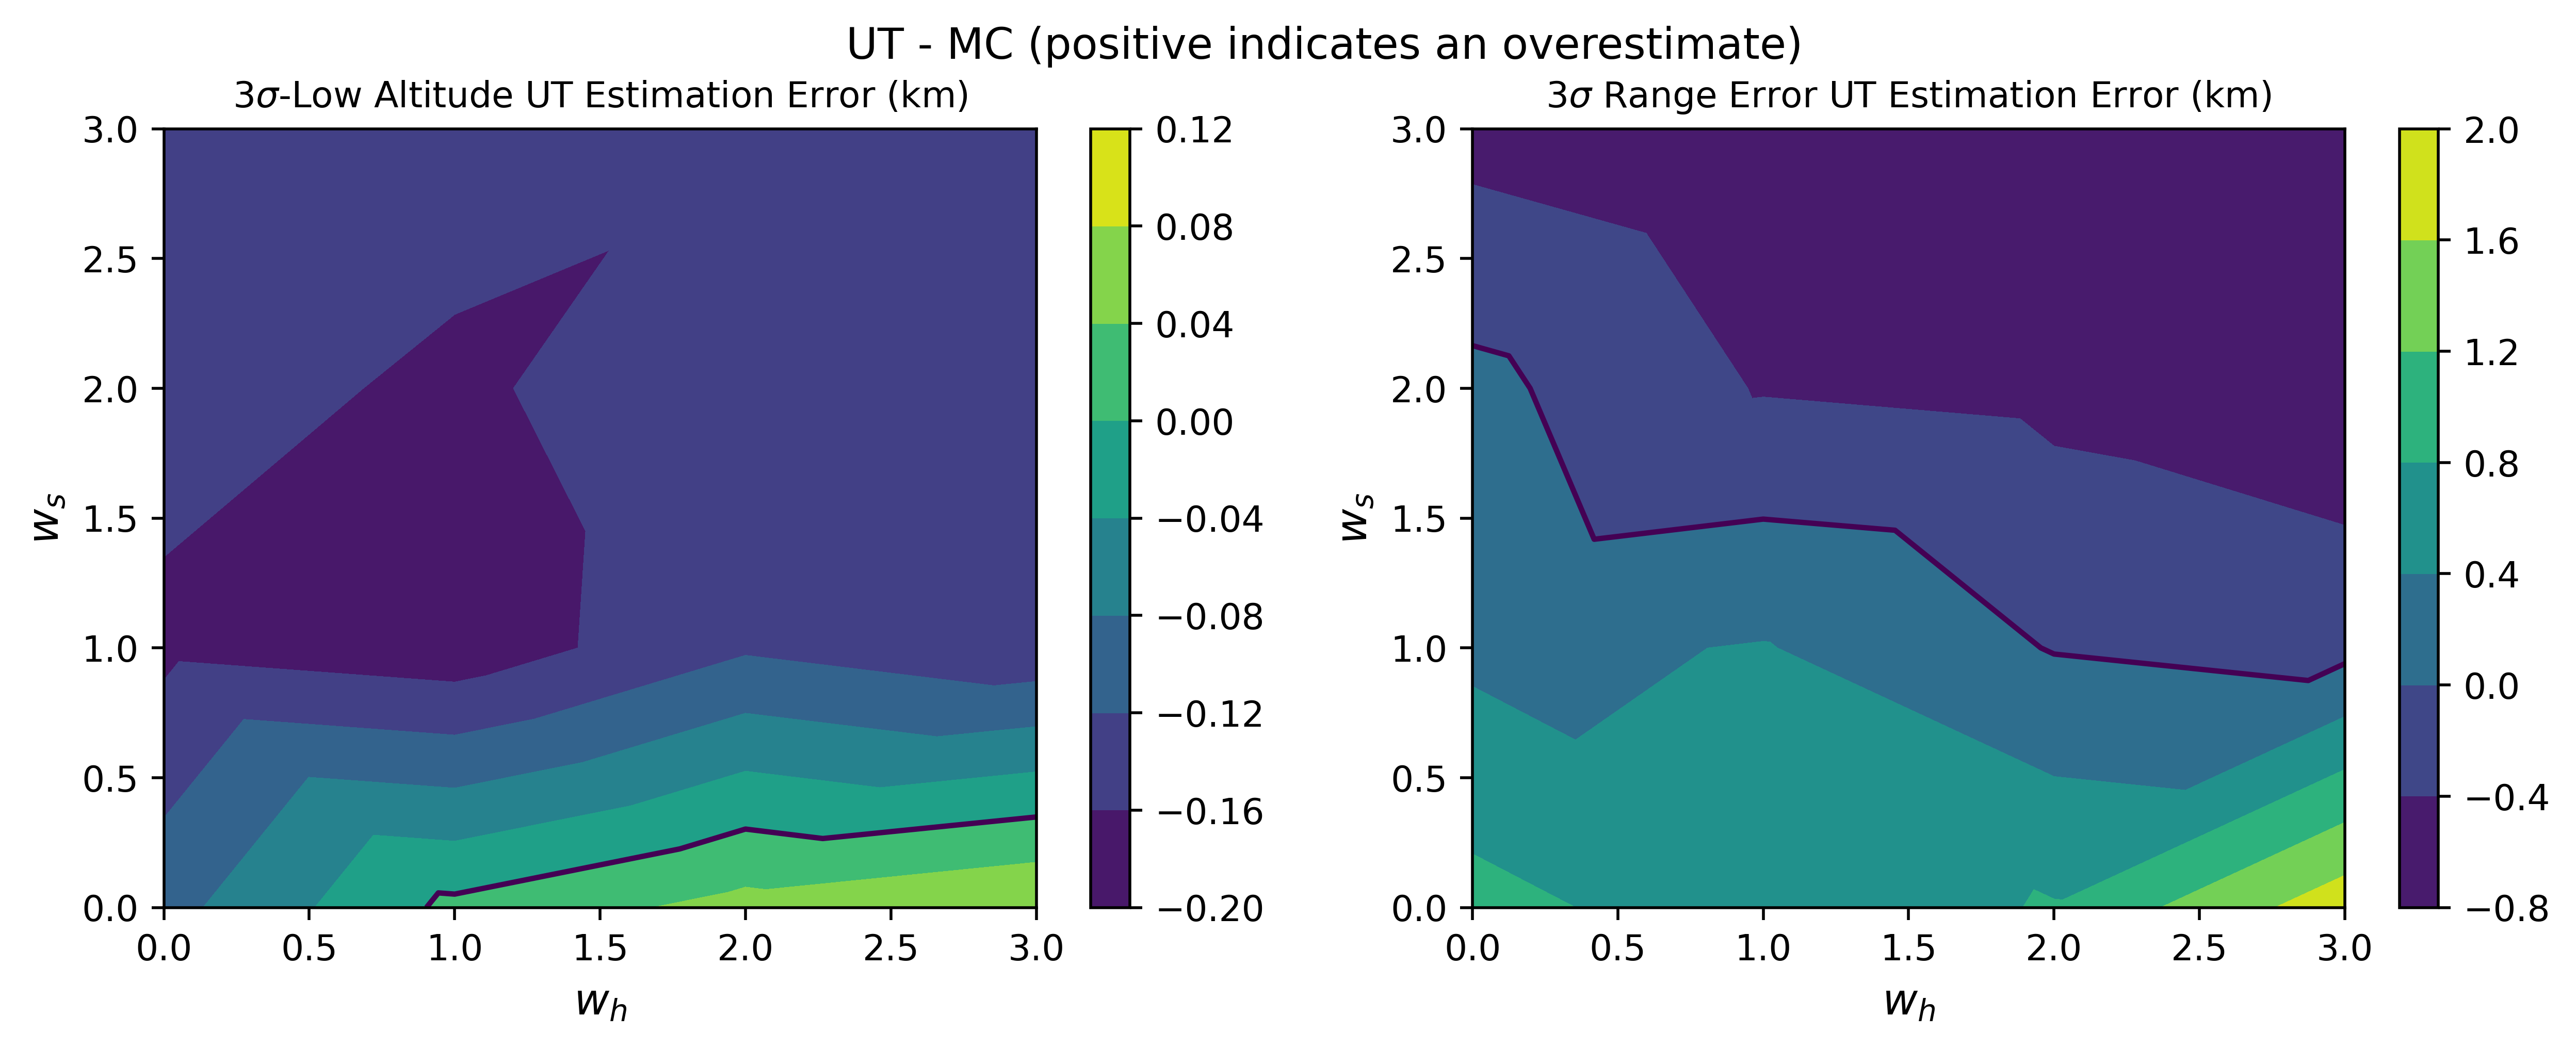
\includegraphics[width=1\textwidth]{Images/Reoptimized_WeightSweepError}
%	\caption{}
%	\label{Fig:MCErrorsOpenLoop}
%\end{figure}

\subsection{Closed-Loop Optimization}
%Maybe show ONLY  Monte Carlo results here. Then in the next section, do a detailed comparison. Justified by the fact that optimized gains are what we would want to use, so we should confirm those? But MC here already confirms. We could maybe get away with showing the UT only
Figure~\ref{Fig:MCResultsFixedGain} presents contours of the Monte Carlo estimated 3$\sigma$-low altitude and range errors for the closed-loop guidance with $K=K_2$. Introducing feedback allows the guidance to achieve 3$\sigma$ range errors as low as 5.6 km while also keeping the 3$\sigma$-low altitude above 9 km. Figure~\ref{Fig:MCErrorsFixedGain} shows the contours of the errors in the UT statistics compared to the Monte Carlo results. The error in 3$\sigma$-low altitude varies between 120 m overestimate and a 360 underestimate. For a majority of $(w_h,w_s)$ pairs, the low altitude is underestimated. 
\begin{figure}[h!]
	\centering
	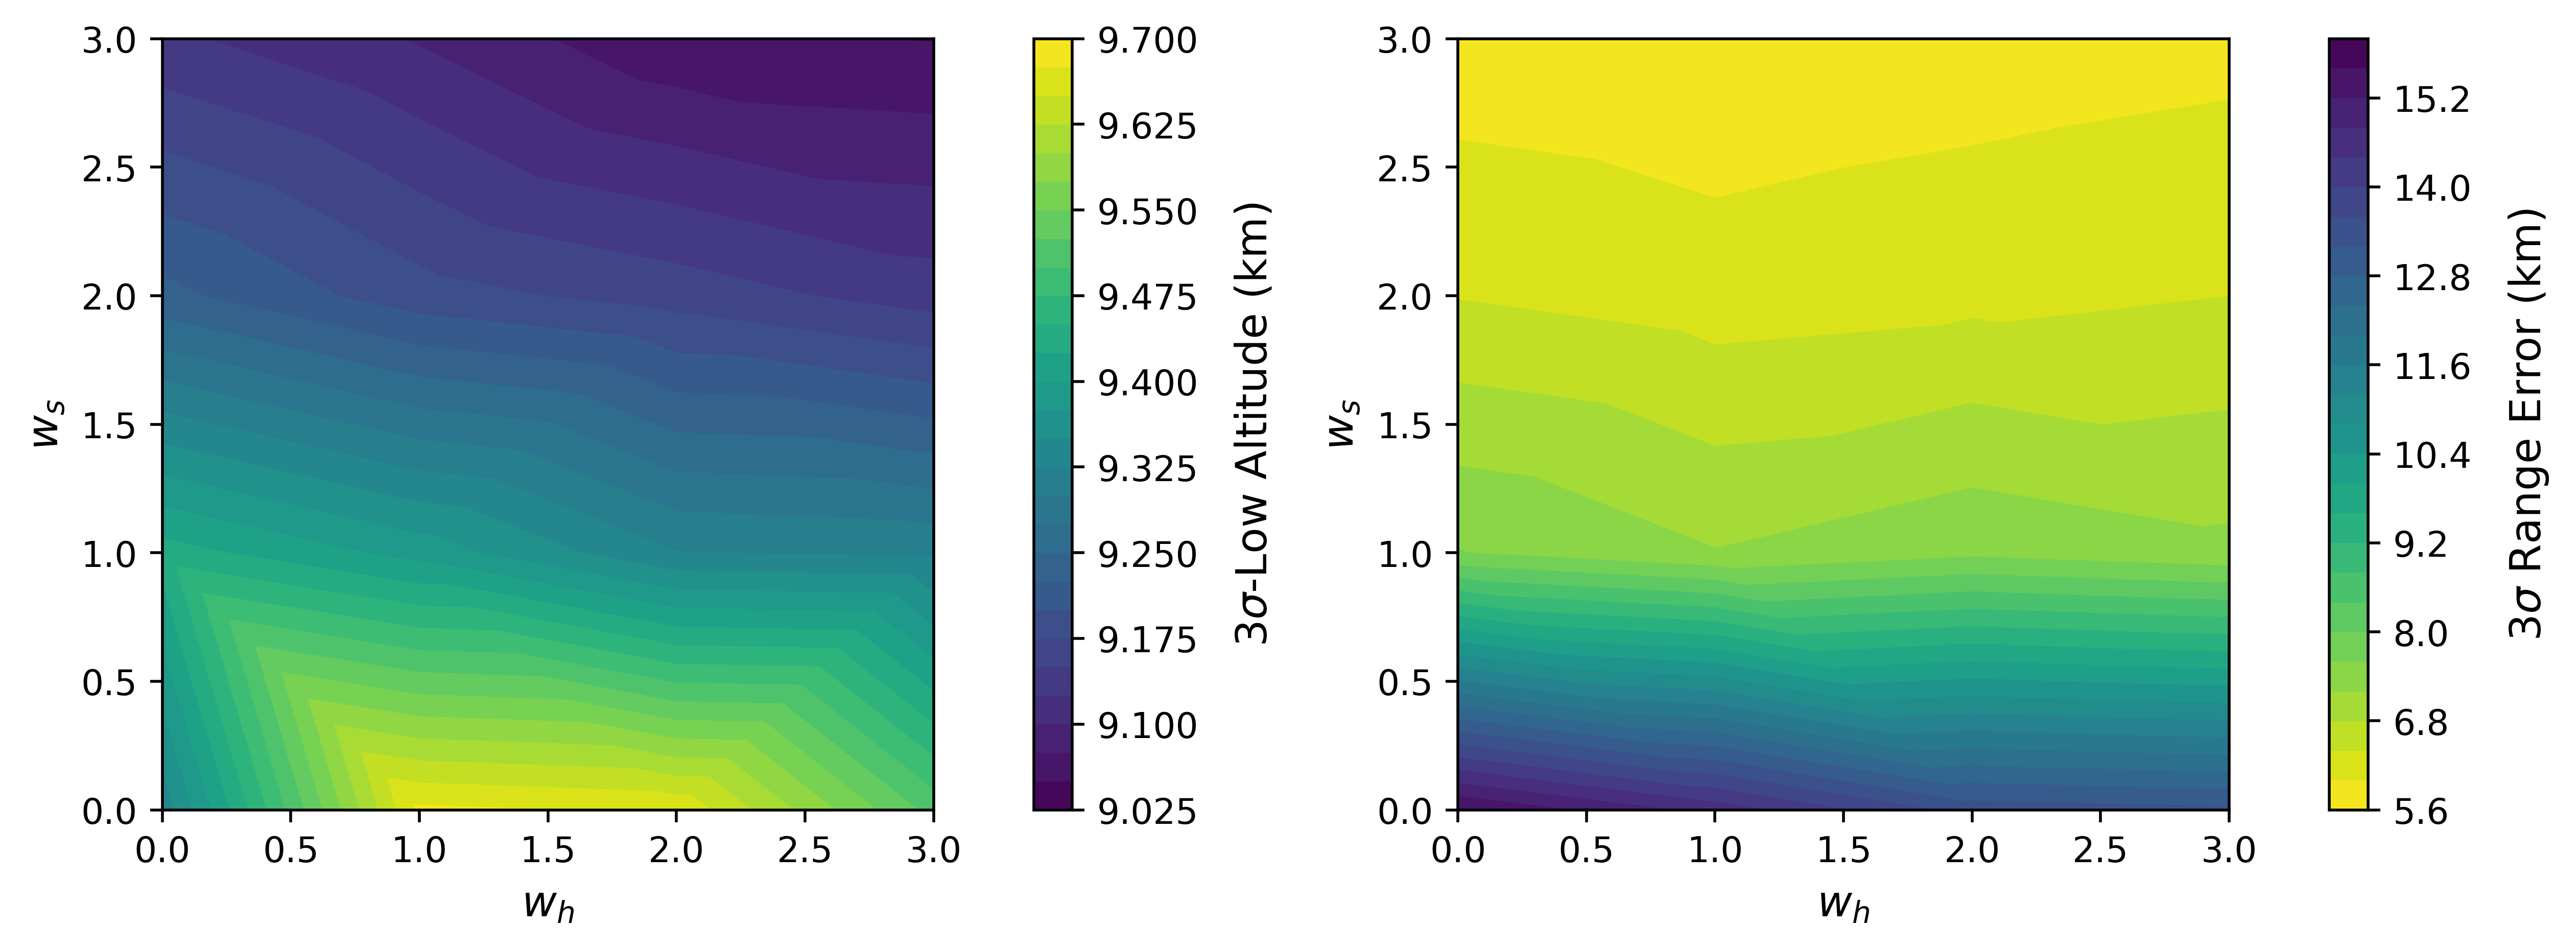
\includegraphics[width=1\textwidth]{Images/Reestimated_WeightSweepMCResults}
	\caption{Monte Carlo statistics for the closed-loop trajectory optimization with static gains.}
	\label{Fig:MCResultsFixedGain}
\end{figure}
\begin{figure}[h!]
	\centering
	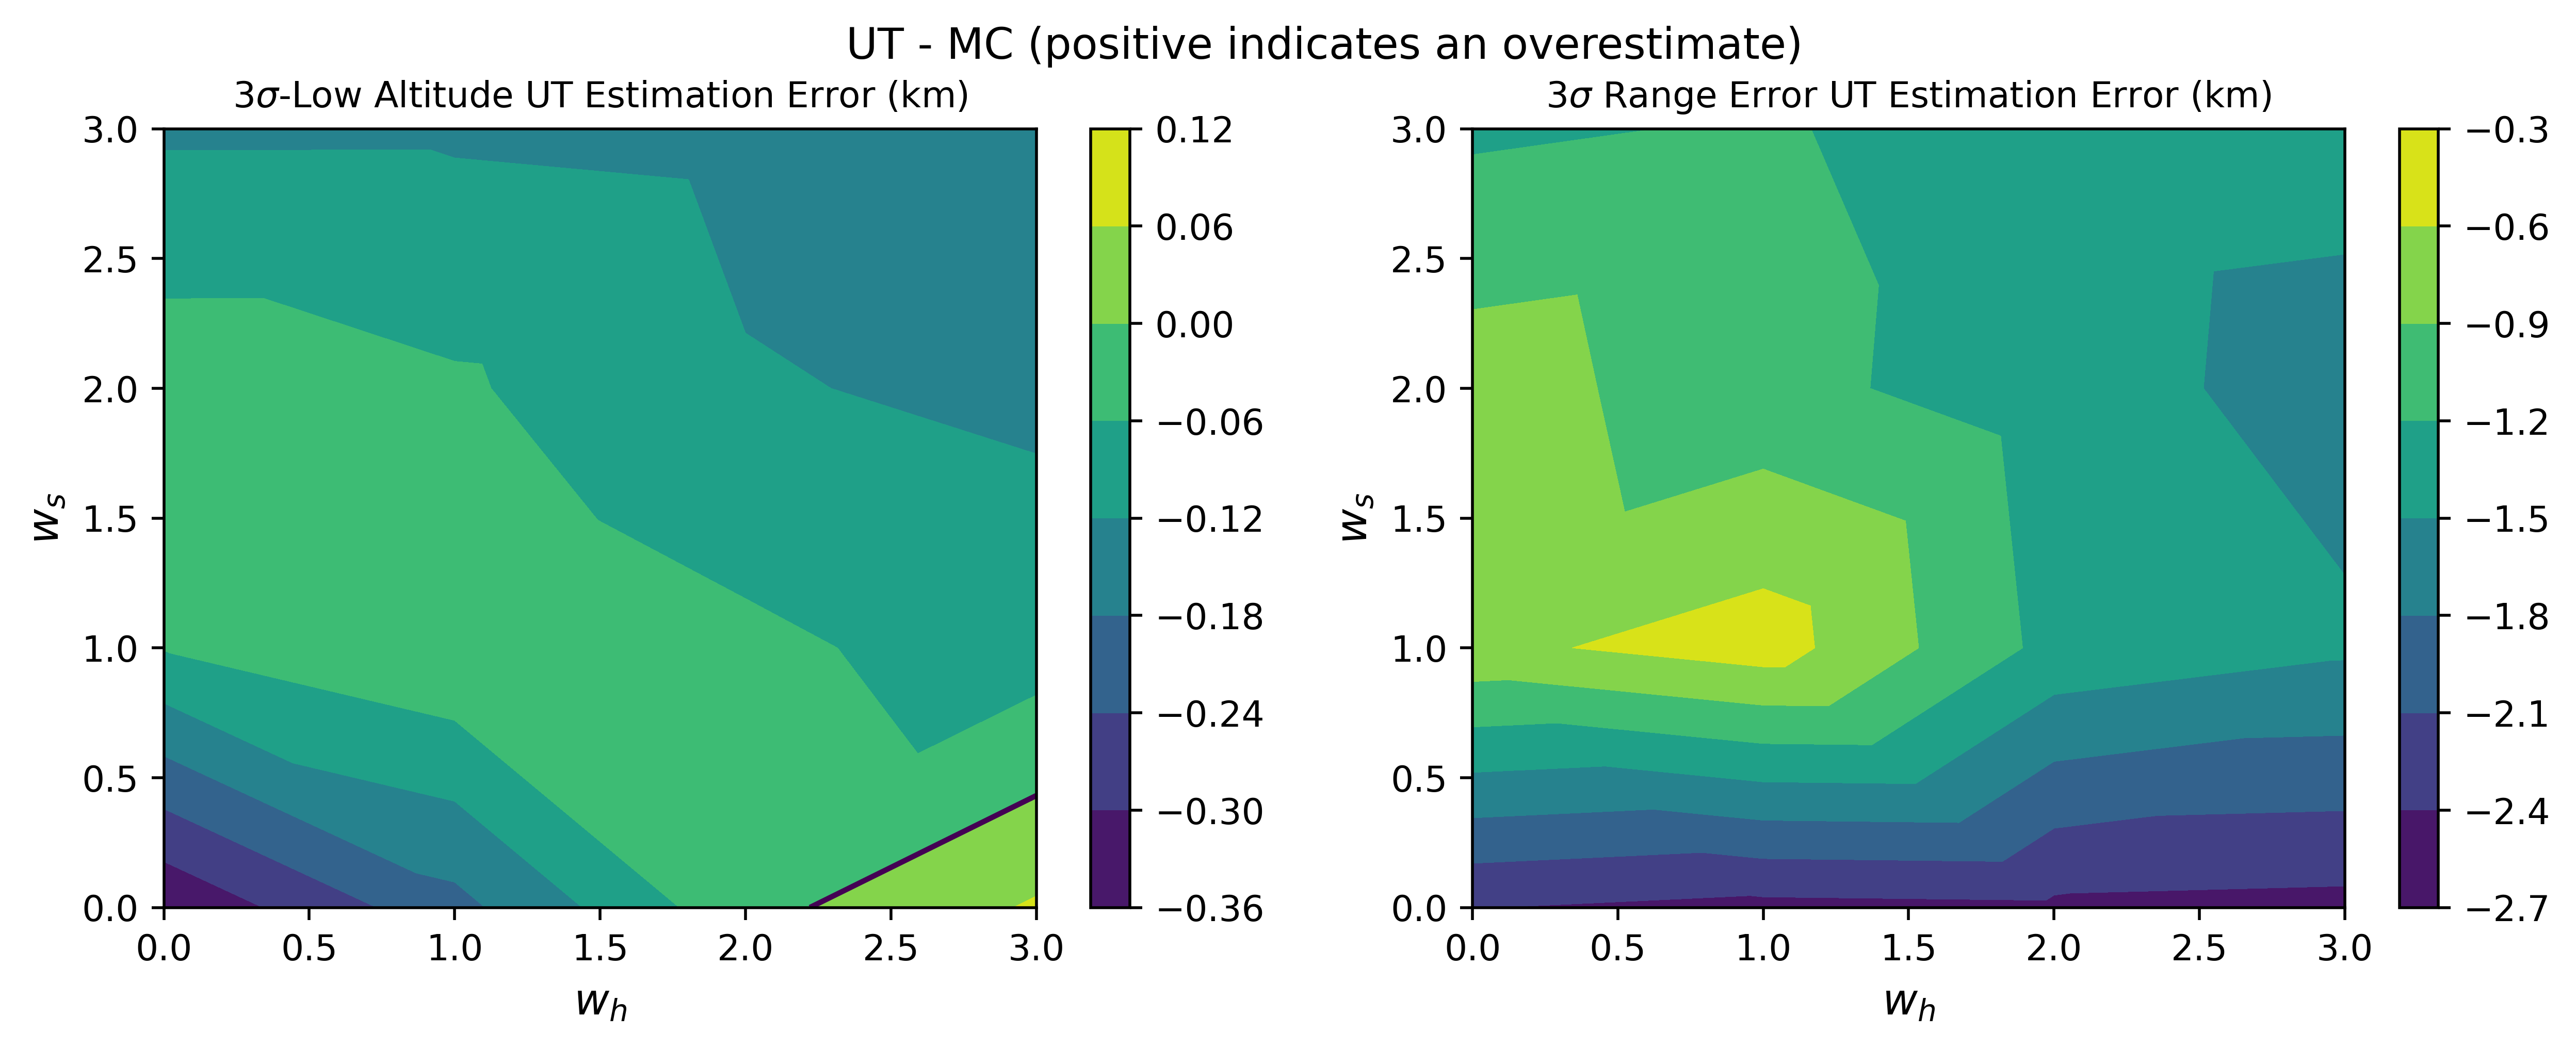
\includegraphics[width=1\textwidth]{Images/Reestimated_WeightSweepError}
	\caption{Unscented Transform estimation errors relative to Monte Carlo statistics for trajectory optimization with static feedback gains.}
	\label{Fig:MCErrorsFixedGain}
\end{figure}


\section{Joint Gain Optimization}
%Motivate the constant gain optimization here by showing an example of bad MC performance when simultaneously optimizing velocity-varying gains? Then show how well the constant gains can do when jointly optimized. 

In this section, the ROGP is again solved for a variety of weights but now the gains are treated as design parameters, and the DDP modification presented in Subsection~\ref{Sec:DesignOptimization} is used to jointly optimize them alongside the reference trajectory and control. As one might intuitively expect, the effect is much more extreme with joint optimization. 

An additional 800 meters of low altitude can be achieved (relative to the previous unoptimized gains), but at the expense of huge range errors. However, a very tight range distribution of $3\sigma_s = 3$ km can be achieved while still maintaining a 9 km 3$\sigma$-low altitude.  
\begin{figure}[h!]
	\centering
	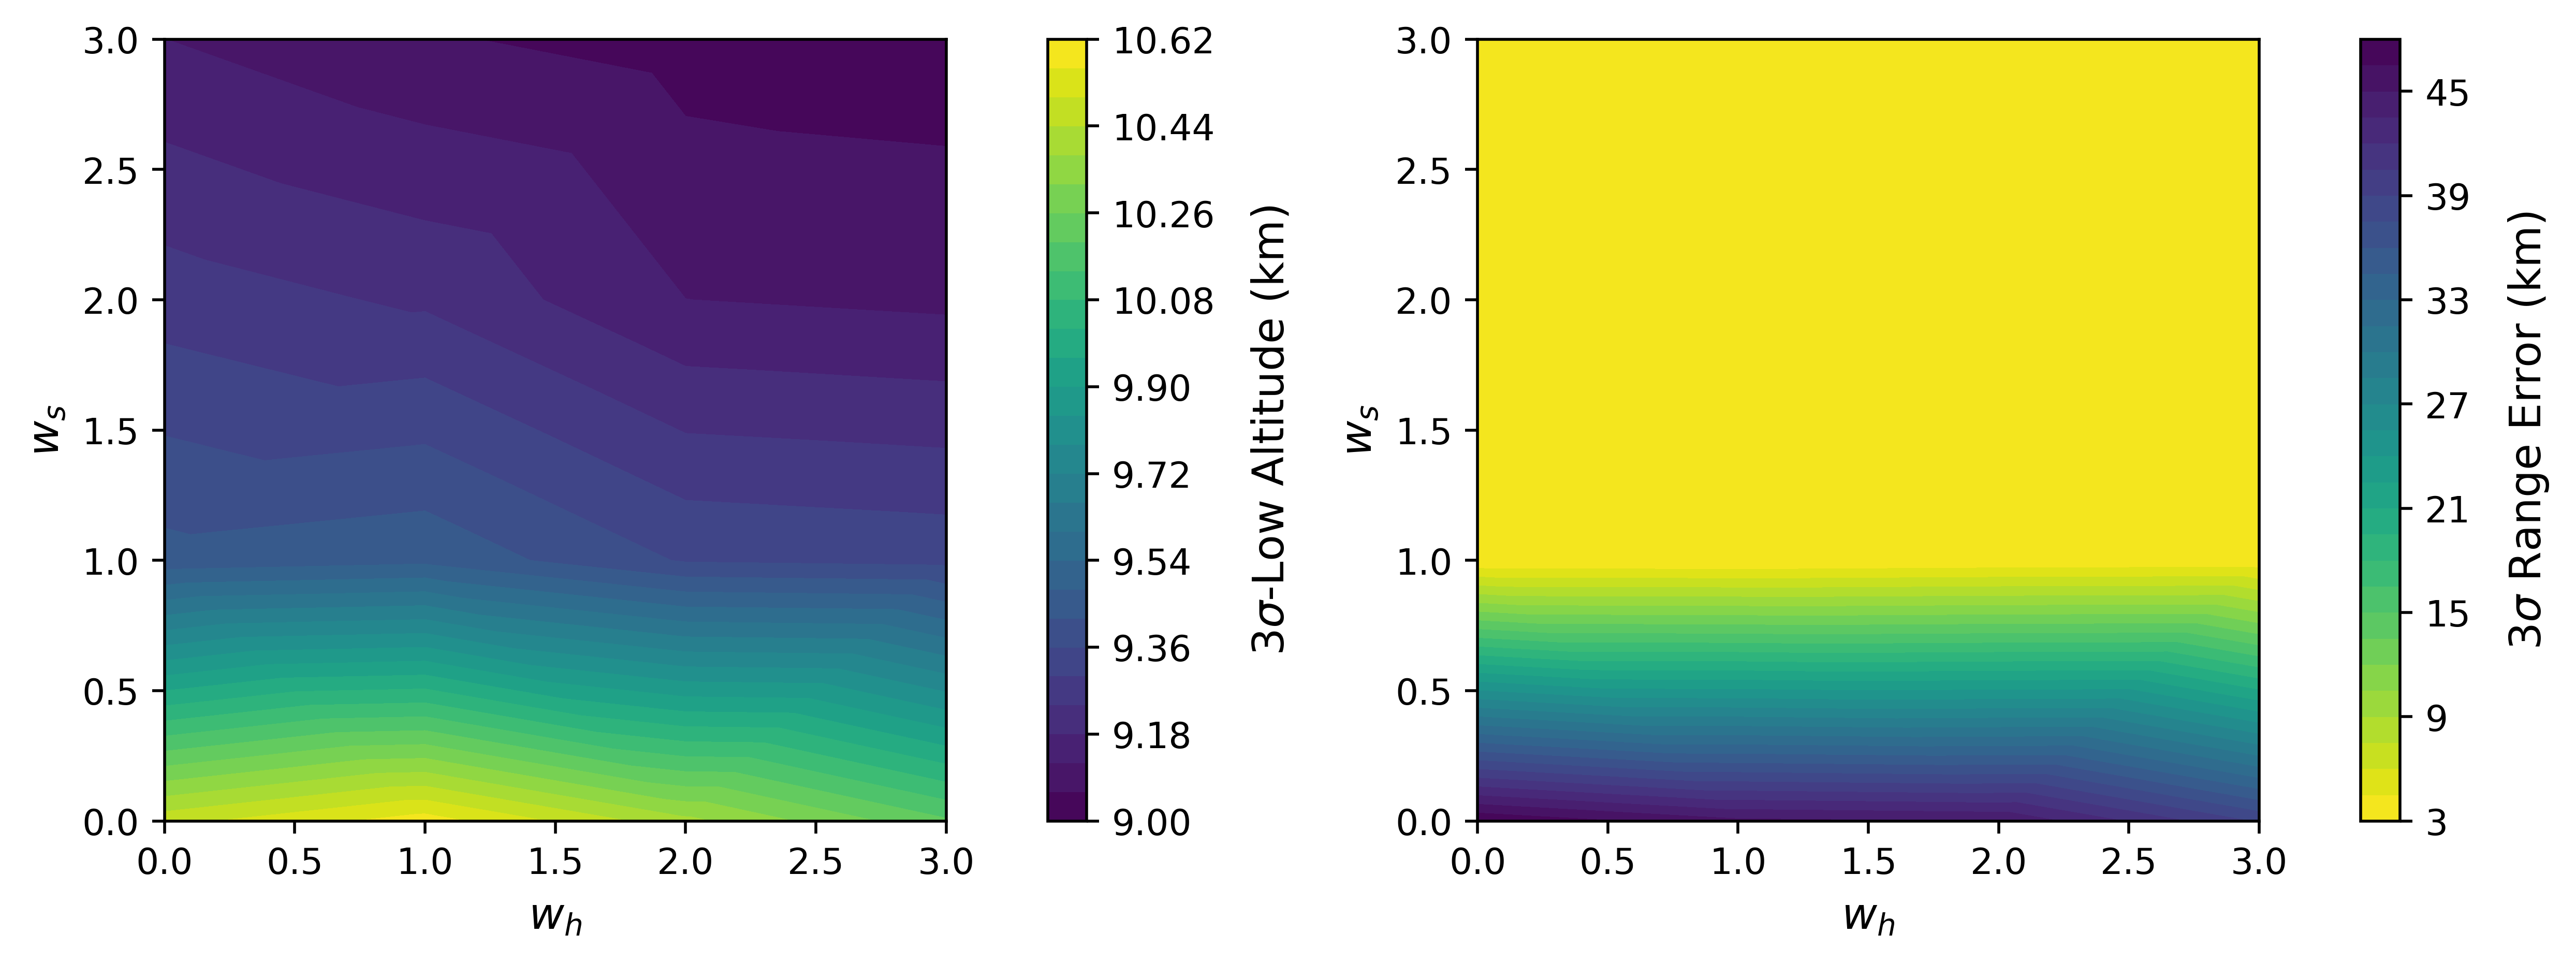
\includegraphics[width=1\textwidth]{Images/Reoptimized_WeightSweepMCResults}
	\caption{Monte Carlo statistics for jointly optimized static feedback gains.}
	\label{Fig:MCResultsOptGain}
\end{figure}
\begin{figure}[h!]
	\centering
	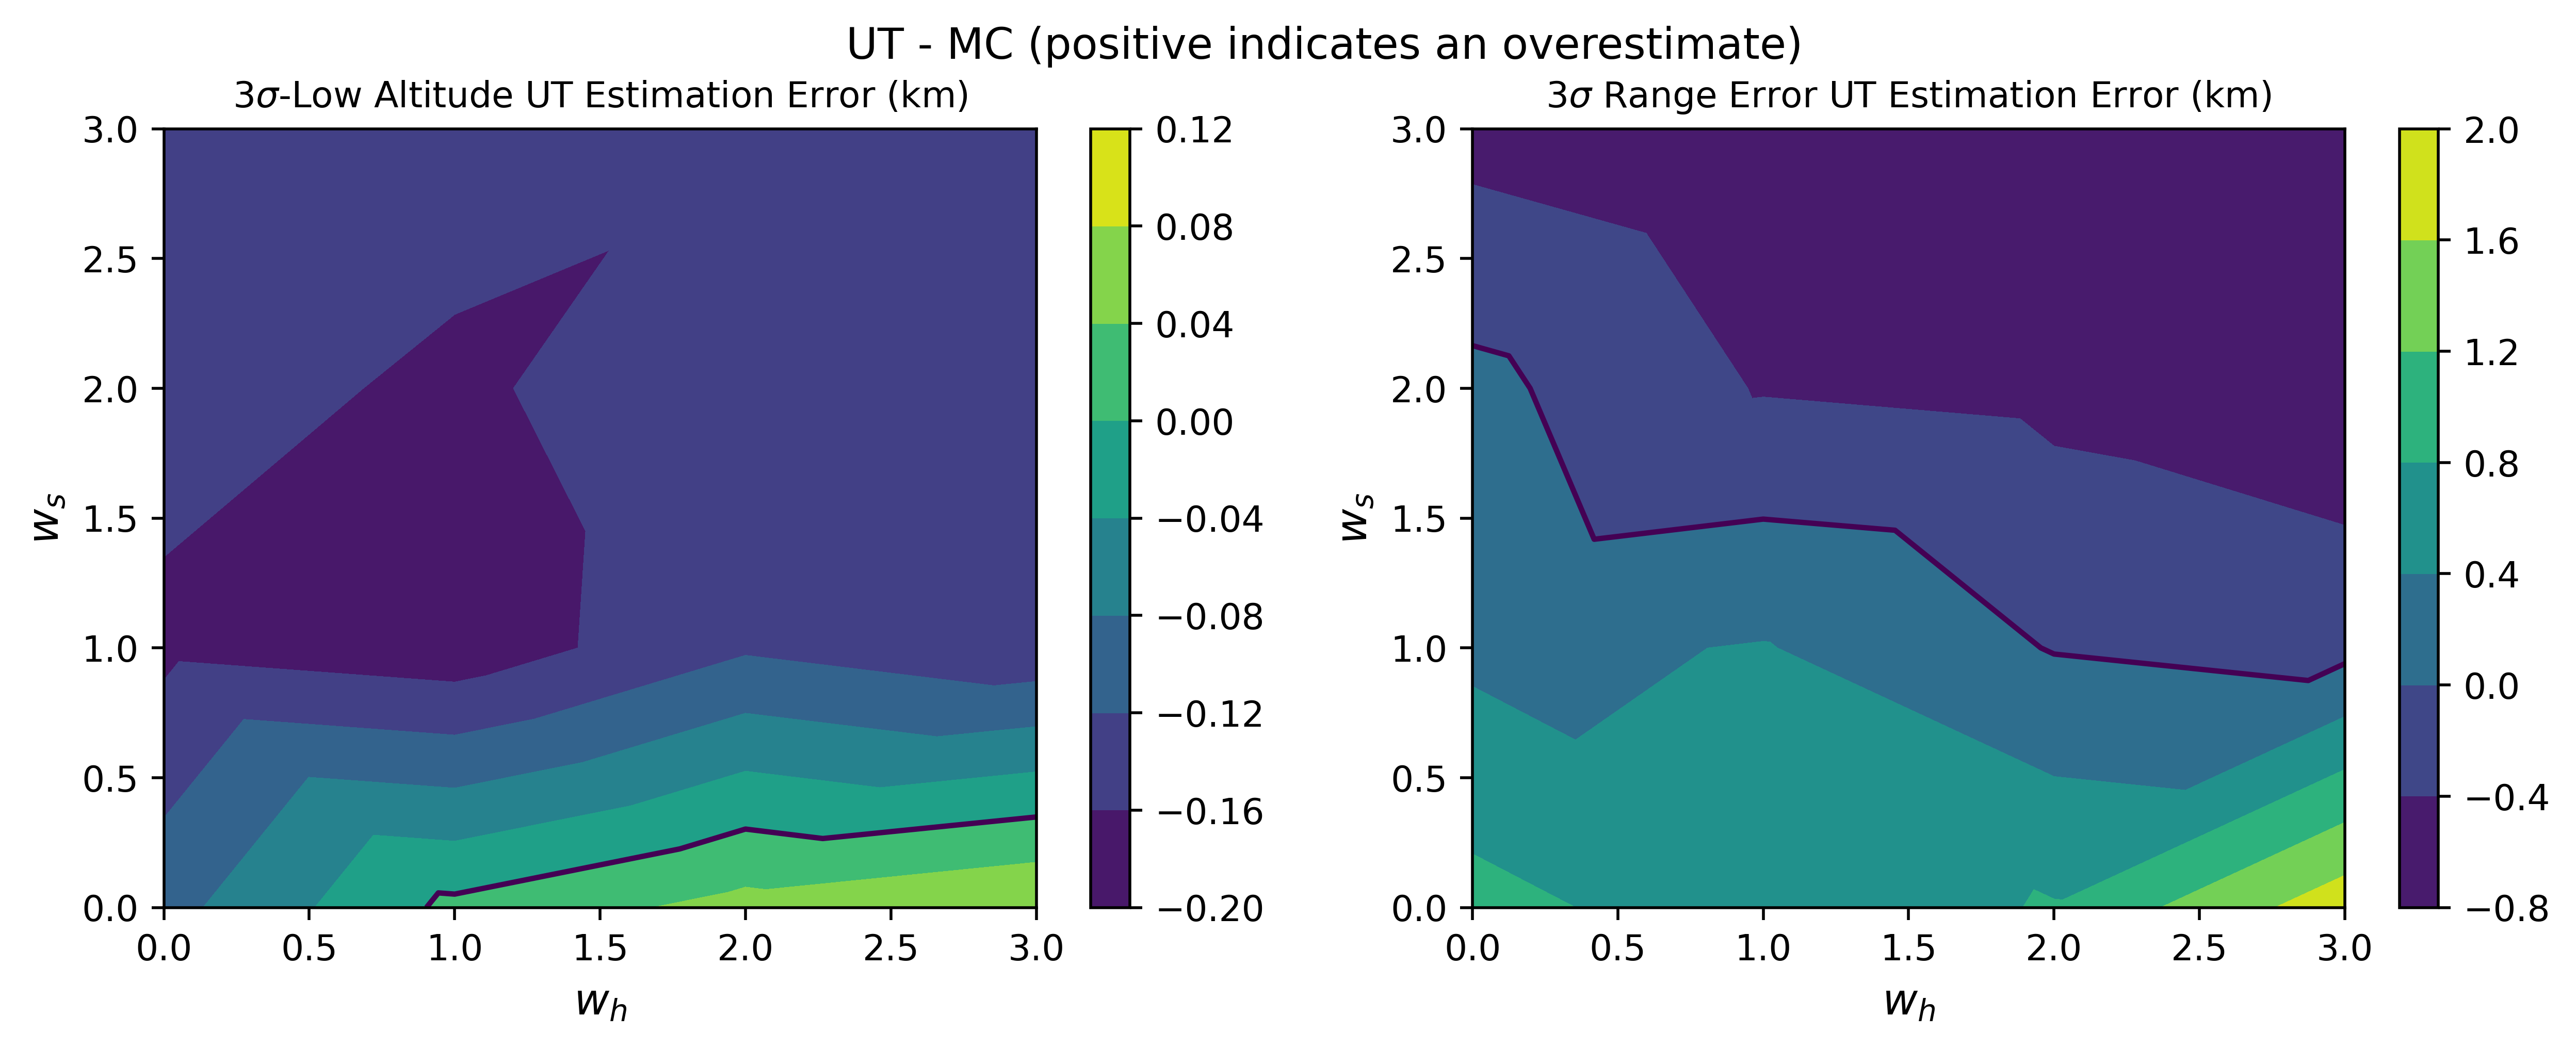
\includegraphics[width=1\textwidth]{Images/Reoptimized_WeightSweepError}
	\caption{Unscented Transform estimation errors relative to Monte Carlo statistics for jointly optimized static feedback gains.}
	\label{Fig:MCErrorsOptGain}
\end{figure}
%TODO: plot mean (=target) range to determine if longer or shorter trajectories are more robust. 

\section{Detailed Comparison}
Other sections are input-output, examining the tradeoffs enabled by varying the weights in the performance index. In this section we present an in-depth look at a single solution, including visualizing the samples over time. We also perform further analysis to determine which uncertainties most strongly affect performance by applying the global sensitivity analysis technique known as Monte Carlo Filtering \cite{MonteCarloFiltering}. 

%TODO


\section{Convergence}
In this section we examine the convergence of solutions using the full DDP algorithm, with the $\mathbf{f}_{\state\state}=\zero,\, \mathbf{f}_{\control\state}=\zero$ modification proposed in Subsection~\ref{Sec:DDP_Simplification}, and the iterated Linear Quadratic Regulator (iLQR) variation where additionally $\mathbf{f}_{\control\control}=\zero$. We solve the ROGP for $w_h=w_s=1$ with each method. The primary metrics that we are interested in are the total cost, the total number of iterations, the time spent computing derivatives, and the maximum of the norm of the gradient of the value function with respect to the controls over the entire trajectory. We will also examine the linesearch stepsizes and regularization parameters.
%Have to remove either state or parameter uncertainty to be able to use the full derivatives formulation.

\begin{figure}[h!]
	\centering
	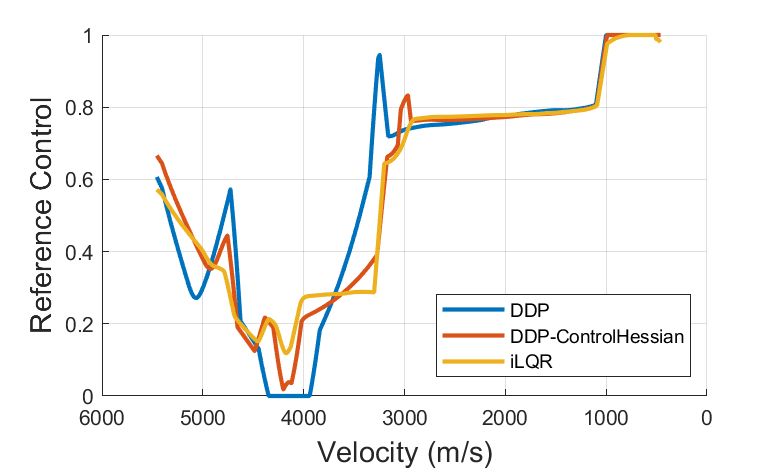
\includegraphics[width=1\textwidth]{Images/Convergence/ControlProfiles}
	\caption{Total cost per iteration}
	\label{Fig:ConvergeControls}
\end{figure}
\begin{figure}[h!]
	\centering
	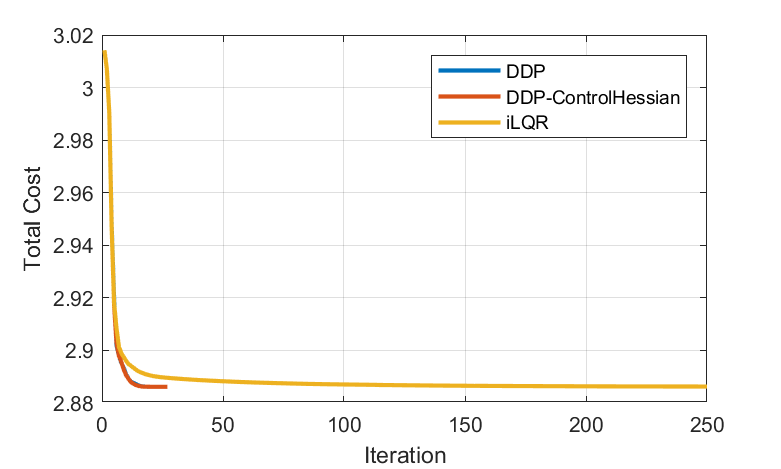
\includegraphics[width=1\textwidth]{Images/Convergence/cost}
	\caption{Total cost per iteration}
	\label{Fig:ConvergeCost}
\end{figure}
\begin{figure}[h!]
	\centering
	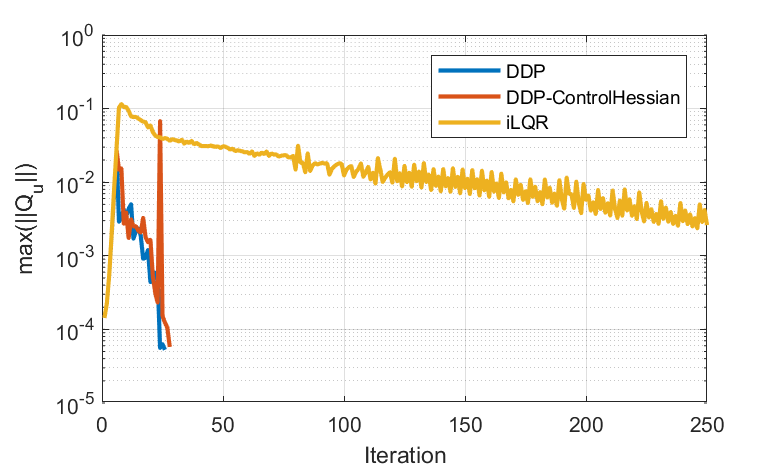
\includegraphics[width=1\textwidth]{Images/Convergence/grad_norm}
	\caption{Maximum control gradient norm over all timesteps.}
	\label{Fig:ConvergeGradient}
\end{figure}
\begin{figure}[h!]
	\centering
	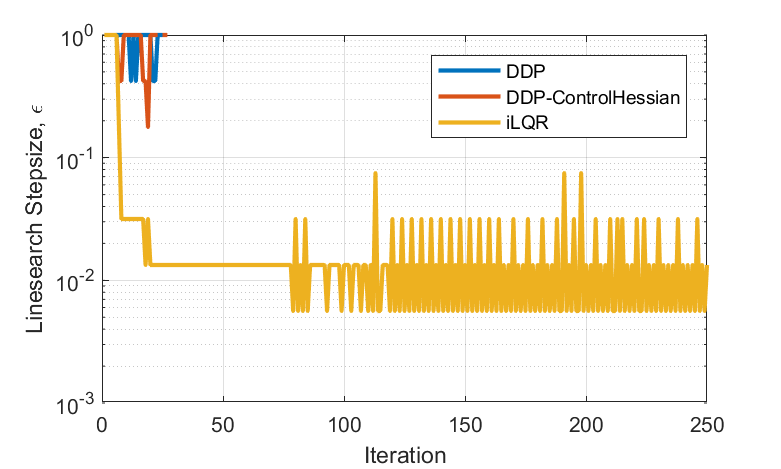
\includegraphics[width=1\textwidth]{Images/Convergence/alpha}
	\caption{Backtracking linesearch stepsize per iteration.}
	\label{Fig:ConvergeStepsize}
\end{figure}
\begin{figure}[h!]
	\centering
	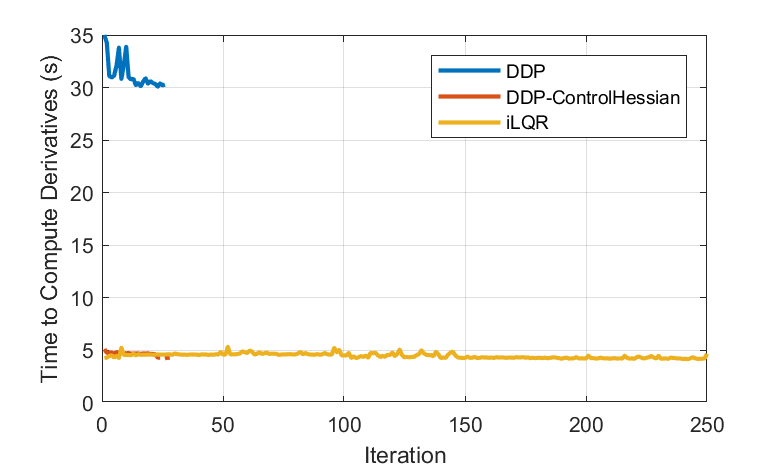
\includegraphics[width=1\textwidth]{Images/Convergence/time_derivs}
	\caption{Time in seconds spent computing derivatives of the cost and dynamics at each iteration.}
	\label{Fig:ConvergeTime}
\end{figure}
%TODO: SHow control profiles? All three converge to similar but not exactly the same profile. 
Figure~\ref{Fig:ConvergeStepsize} shows the total cost at each iteration. Full DDP achieves the lowest cost of $2.864$ after 81 iterations. Control Hessian-only DDP achieves a cost of 2.870 after 46 iterations, and iLQR has the highest cost, 2.871, and still has not converged after 250 iterations. Figure~\ref{Fig:ConvergeGradient} shows the maximum gradient at each iteration. The iLQR solution does not appear to reach a stationary point. 
Figure~\ref{Fig:ConvergeStepsize} shows the stepsizes accepted in the linesearch procedure. Both DDP variants frequently accepted the full step $\epsilon=1$, while iLQR always took considerably smaller steps on the order of $ 10^{-2} $. Finally, Fig.~\ref{Fig:ConvergeTime} shows the drastic, nearly 10x reduction in time spent computing the derivatives resulting from omitting Hessian terms. The average times were $47.7$ s, 5.6 s, and 5.2 s, respectively. 
This example shows that retaining the second order derivatives with respect to the controls achieves nearly the same convergence as the full DDP algorithm while being only mildly more expensive to compute than the iLQR solution. 

%TODO: sensitivity to initial guess? 

%\section{Joint Optimization of Velocity-Varying Gains}
%Show negative result and describe overfitting problem. 

%\section{As Vehicle Design Tool}
%What L/D is required to achieve similar entry altitudes for a heavier vehicle of $\beta=200$? We use a simple scaling of the L/D profile $L/D$. The gains are jointly optimized, and additionally, the entry flight path angle is treated as a design variable. To estimate a useful lower bound on the L/D, we select $w_h=3, w_s=0$; the desired solution will likely place non-zero weight on the range errors, and thus need even more L/D. 
%%% Local Variables: ***
%%% mode: latex ***
%%% TeX-master: "thesis.tex" ***
%%% End: ***
